\newpage

\section{Le Théorème Central Limite (TCL)}

\subsection{Introduction : L'omniprésence de la loi normale}

Dans la section précédente, la Loi des Grands Nombres (LLN) nous a donné une garantie fondamentale : la moyenne d'échantillon $\bar{X}_n$ converge vers la vraie moyenne $\mu$ lorsque $n$ devient grand.
$$ \bar{X}_n \xrightarrow{p.s.} \mu $$
La LLN nous dit \textbf{où} la moyenne d'échantillon converge (vers la constante $\mu$), mais elle ne nous dit rien sur la \textit{forme} de la distribution de $\bar{X}_n$ autour de $\mu$ pour un $n$ grand, mais fini.

Le \textbf{Théorème Central Limite (TCL)} comble cette lacune. Il décrit la \textit{manière} dont $\bar{X}_n$ converge, en nous donnant la forme de sa distribution. C'est sans doute le théorème le plus important des statistiques.

\begin{intuitionbox}[L'Idée Fondamentale]
Intuitivement, ce résultat affirme qu'une \textbf{somme} d'un grand nombre de variables aléatoires indépendantes et identiquement distribuées (i.i.d.) tend, le plus souvent, à suivre une \textbf{loi normale} (aussi appelée loi de Laplace-Gauss ou "courbe en cloche").

Ce théorème et ses généralisations offrent une explication à l'omniprésence de la loi normale dans la nature. De nombreux phénomènes (la taille d'un individu, l'erreur de mesure d'un instrument, le bruit de fond d'un signal) sont le résultat de l'addition d'un très grand nombre de petites perturbations aléatoires. Le TCL nous dit que le résultat de cette somme sera, inévitablement, distribué selon une loi normale.
\end{intuitionbox}

\subsection{L'illustration : la somme des "Pile ou Face"}

Prenons l'exemple le plus simple pour illustrer ce phénomène : le jeu de "pile ou face".



\begin{examplebox}[Distribution de la Somme de $n$ Lancers]
Soit $X_i$ le résultat du $i$-ème lancer, avec $X_i = 1$ pour "Face" (probabilité 0,5) et $X_i = 0$ pour "Pile" (probabilité 0,5). La distribution d'origine (pour $n=1$) n'est pas du tout une courbe en cloche : c'est une distribution discrète avec deux bâtons de même hauteur.

Considérons la \textbf{somme} $S_n = X_1 + X_2 + \dots + X_n$, qui représente le nombre total de "Face" obtenus en $n$ lancers.

\begin{itemize}
    \item \textbf{Pour $n=1$ :} La distribution de $S_1$ est :
    \begin{itemize}
        \item Valeurs de la somme : \{0, 1\}
        \item Fréquences : \{0.5, 0.5\}
    \end{itemize}
    
    \item \textbf{Pour $n=2$ :} Les sommes possibles sont \{0, 1, 2\}. La distribution de $S_2$ est :
    \begin{itemize}
        \item Valeurs de la somme : \{0, 1, 2\}
        \item Fréquences : \{0.25, 0.5, 0.25\} (elle forme un triangle).
    \end{itemize}
    
    \item \textbf{Pour $n=3$ :} Les sommes possibles sont \{0, 1, 2, 3\}. La distribution de $S_3$ est :
    \begin{itemize}
        \item Valeurs de la somme : \{0, 1, 2, 3\}
        \item Fréquences : \{0.125, 0.375, 0.375, 0.125\}
    \end{itemize}
\end{itemize}

\begin{center}
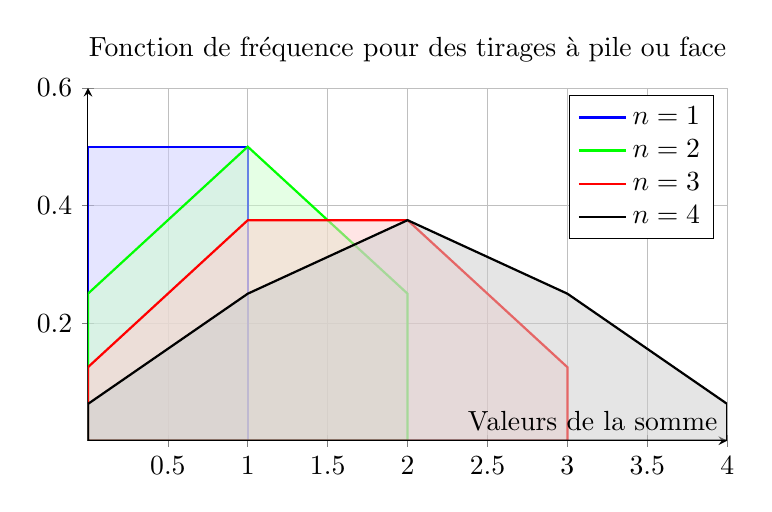
\begin{tikzpicture}
  \begin{axis}[
    width=0.8\textwidth,
    height=0.5\textwidth,
    xlabel={Valeurs de la somme},
    title={Fonction de fréquence pour des tirages à pile ou face},
    grid=both,
    grid style={line width=.1pt, draw=gray!30},
    major grid style={line width=.2pt,draw=gray!50},
    domain=0:4,
    samples=100,
    enlargelimits=false,
    axis lines=middle,
    xmin=0, xmax=4,
    ymin=0, ymax=0.6
  ]
  % n=1
  \addplot [thick, color=blue, fill=blue!20, fill opacity=0.5] coordinates {(0,0.5) (1,0.5)} \closedcycle;
  % n=2
  \addplot [thick, color=green, fill=green!20, fill opacity=0.5] coordinates {(0,0.25) (1,0.5) (2,0.25)} \closedcycle;
  % n=3
  \addplot [thick, color=red, fill=red!20, fill opacity=0.5] coordinates {(0,0.125) (1,0.375) (2,0.375) (3,0.125)} \closedcycle;
  % n=4 (suggéré)
  \addplot [thick, color=black, fill=black!20, fill opacity=0.5] coordinates {(0,0.0625) (1,0.25) (2,0.375) (3,0.25) (4,0.0625)} \closedcycle;
  
  \legend{$n=1$,$n=2$,$n=3$,$n=4$}
  \end{axis}
\end{tikzpicture}
\end{center}

Graphiquement, on constate que plus le nombre de tirages $n$ augmente (par exemple, jusqu'à $n=12$), plus la courbe de fréquence (qui reste discrète) se rapproche d'une courbe en cloche symétrique, caractéristique de la loi normale.
\end{examplebox}

\subsection{Distribution de la population vs. Distribution d'échantillonnage}

Le point le plus remarquable du TCL est qu'il fonctionne \textit{quelle que soit} la distribution de départ.

\begin{intuitionbox}[Population vs. Échantillonnage]
Imaginez deux univers de distributions :

\begin{itemize}
    \item \textbf{1. La Distribution de la Population ($X_i$) :} C'est la loi de nos variables $X_i$ individuelles. Elle peut avoir \textbf{n'importe quelle forme} (par exemple, une distribution bimodale, asymétrique, ou uniforme). Cette distribution a une "vraie" moyenne $\mu$ et un "vrai" écart-type $\sigma$.
    
    \item \textbf{2. La Distribution d'Échantillonnage ($\bar{X}_n$) :} C'est la distribution de la \textit{moyenne} $\bar{X}_n = (X_1 + \dots + X_n)/n$, calculée sur des échantillons de taille $n$. C'est la distribution de "toutes les moyennes d'échantillon possibles".
\end{itemize}

Le TCL énonce la relation magique entre les deux :

\textbf{Quelle que soit la forme de la distribution de la population, plus la taille de l'échantillon $n$ croît, plus la distribution d'échantillonnage de la moyenne $\bar{X}_n$ est proche d'une loi normale (gaussienne).}

De plus, les paramètres de cette loi normale sont :
\begin{itemize}
    \item \textbf{Moyenne :} La distribution de $\bar{X}_n$ est centrée sur la même moyenne $\mu$ que la population.
    \item \textbf{Écart-type :} La distribution de $\bar{X}_n$ est beaucoup plus resserrée. Son écart-type (appelé "erreur standard") est $\sigma_{\bar{X}} = \frac{\sigma}{\sqrt{n}}$.
\end{itemize}
Cette dispersion $\sigma/\sqrt{n}$ qui tend vers 0 est la manifestation de la Loi des Grands Nombres. Le TCL précise que la \textit{forme} de cette convergence est gaussienne.
\end{intuitionbox}

\subsection{Énoncé formel du Théorème Central Limite}

Pour énoncer le théorème formellement, nous devons d'abord définir les propriétés de la somme $S_n$ et de la moyenne $\bar{X}_n$.

Soit $X_1, \dots, X_n$ des variables aléatoires i.i.d. avec $E[X_i] = \mu$ et $\text{Var}(X_i) = \sigma^2$.

\begin{itemize}
    \item \textbf{La Somme $S_n = \sum X_i$} :
    \begin{itemize}
        \item Espérance : $E[S_n] = E[\sum X_i] = \sum E[X_i] = n\mu$
        \item Variance : $\text{Var}(S_n) = \text{Var}(\sum X_i) = \sum \text{Var}(X_i) = n\sigma^2$
        \item Écart-type : $\sigma_{S_n} = \sqrt{n\sigma^2} = \sigma\sqrt{n}$
    \end{itemize}
    
    \item \textbf{La Moyenne $\bar{X}_n = S_n / n$} :
    \begin{itemize}
        \item Espérance : $E[\bar{X}_n] = E[S_n / n] = \frac{1}{n} E[S_n] = \frac{1}{n} (n\mu) = \mu$
        \item Variance : $\text{Var}(\bar{X}_n) = \text{Var}(S_n / n) = \frac{1}{n^2} \text{Var}(S_n) = \frac{1}{n^2} (n\sigma^2) = \frac{\sigma^2}{n}$
        \item Écart-type : $\sigma_{\bar{X}_n} = \sqrt{\sigma^2 / n} = \frac{\sigma}{\sqrt{n}}$
    \end{itemize}
\end{itemize}

Nous voyons que la distribution de $S_n$ s'étale (variance $\to \infty$) tandis que celle de $\bar{X}_n$ se contracte (variance $\to 0$). Pour étudier la \textit{forme} de la convergence, nous créons une variable "stable" en la centrant (soustrayant la moyenne) et en la réduisant (divisant par l'écart-type). C'est la variable $Z_n$.

\begin{theorembox}[Théorème Central Limite (Lindeberg-Lévy)]
Soit $X_1, X_2, \dots, X_n$ une suite de variables aléatoires \textbf{i.i.d.} (indépendantes et identiquement distribuées) suivant la même loi $D$.
Supposons que l'\textbf{espérance $\mu$} et l'\textbf{écart-type $\sigma$} de cette loi $D$ existent, sont finis, et $\sigma \neq 0$.

Considérons la variable aléatoire standardisée $Z_n$ :
$$ Z_n = \frac{S_n - E[S_n]}{\sigma_{S_n}} = \frac{S_n - n\mu}{\sigma\sqrt{n}} $$
Cette variable est équivalente à la moyenne standardisée :
$$ Z_n = \frac{\bar{X}_n - E[\bar{X}_n]}{\sigma_{\bar{X}_n}} = \frac{\bar{X}_n - \mu}{\sigma / \sqrt{n}} $$
(Pour tout $n$, $Z_n$ est une variable centrée-réduite : $E[Z_n] = 0$ et $\text{Var}(Z_n) = 1$).

Alors, la suite de variables aléatoires $Z_1, Z_2, \dots, Z_n, \dots$ \textbf{converge en loi} vers une variable aléatoire $Z$ qui suit la \textbf{loi normale centrée réduite $N(0, 1)$}, lorsque $n$ tend vers l'infini.

Cela signifie que si $\Phi$ est la fonction de répartition de la loi $N(0, 1)$, alors pour tout réel $z$ :
$$ \lim_{n \to \infty} P(Z_n \le z) = \lim_{n \to \infty} P\left( \frac{\bar{X}_n - \mu}{\sigma/\sqrt{n}} \le z \right) = \Phi(z) $$
\end{theorembox}